\begin{figure}[htbp]
	\centering
	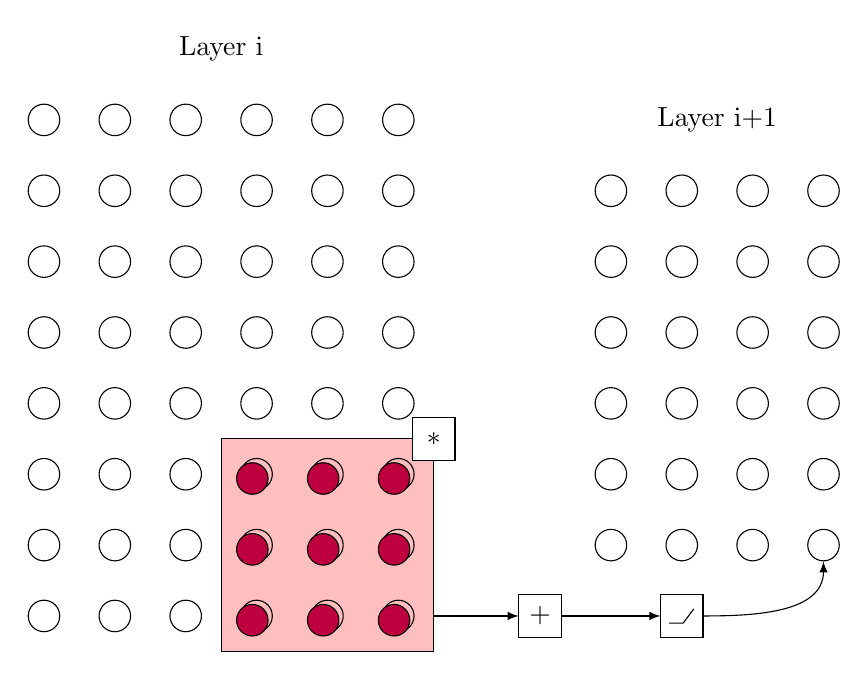
\begin{tikzpicture}[scale=0.9,every path/.style={>=latex}]
		\node (layeri) at (2.5,8) {Layer i};
		\node (layeri) at (9.5,7) {Layer i+1};
     	
     	% draw background for filter
     	\draw[fill=pink] (2.5,2.5) rectangle (5.5,-0.5);
     	
     	% draw rectangle with "*" inside
     	\draw[fill=white] (5.2,2.8) rectangle (5.8,2.2);
     	\node at (5.5,2.5) {$*$};
     	
     	
     	% draw layer 1
     	\foreach \x in {0,...,5}
     	{
     		\foreach \y in {0,...,7}
     		{
     			\node(1-\x-\y) at (\x,\y) [circle,draw,minimum size=0.4cm] {};
     		}
     	}
     	
     	% draw layer 2
     	\foreach \x in {1,...,4}
     	{
     		\foreach \y in {1,...,6}
     		{
     			\node(2-\x-\y) at (\x + 7,\y) [circle,draw,minimum size=0.4cm] {};
     		}
     	}
     	
     	%draw filter
     	\foreach \x in {0,...,2}
     	{
     		\foreach \y in {3,...,5}
     		{
     			\node(f-\x-\y) at (\x - 0.06 + 3,\y - 0.06 - 3) [circle,draw,fill=purple,minimum size=0.4cm] {};
     		}
     	}
     	
     	% draw line from filter to "+" rectangle
     	\draw[->] (5.5,0) to (6.7,0);
     	
     	% draw "+" rectangle
     	\draw[fill=white] (6.7,0.3) rectangle (7.3,-0.3);
     	\node at (7,0) {$+$};
     	
     	% draw line from "+" rectangle to ReLU rectangle
     	\draw[->] (7.3,0) to (8.7,0);
     	
     	% draw ReLU rectangle
     	\draw[fill=white] (8.7,0.3) rectangle (9.3,-0.3);
     	\draw[->,out=0,in=270] (9.3,0) to (2-4-1);
     	\draw[-] (8.82,-0.1) to (9.02,-0.1) to (9.17,0.1);
	\end{tikzpicture}
	\caption{Functioning of a convolutional layer}
	\label{fig:centered_filter}
\end{figure}
